%beamer

%\PassOptionsToClass{handout}{beamer}

% \newboolean{handoutmode}
% \setboolean{handoutmode}{false}
%\newcommand{\handoutmode}{}

%% LaTeX-Beamer template for KIT design
%% by Erik Burger, Christian Hammer
%% title picture by Klaus Krogmann
%%
%% version 2.1
%%
%% mostly compatible to KIT corporate design v2.0
%% http://intranet.kit.edu/gestaltungsrichtlinien.php
%%
%% Problems, bugs and comments to
%% burger@kit.edu
\ifdefined \handoutmode
\documentclass[18pt, handout]{beamer}
\else
\documentclass[18pt]{beamer}
\fi

\usepackage[T1]{fontenc}
\usepackage[utf8]{inputenc}

\usepackage{../preamble/templates/beamerthemekit}

\usepackage[vlined]{algorithm2e}  %possible: noend, noline, ...
\usepackage{amssymb}
\usepackage{amsmath}
\usepackage{wasysym}
\usepackage{graphicx}
%\usepackage{hyperref}
\usepackage[export]{adjustbox}
\usepackage{wrapfig}
\usepackage{colortbl}
\usepackage{tikz}
\usetikzlibrary{matrix}
\usetikzlibrary{arrows.meta}
\usetikzlibrary{automata}
\usetikzlibrary{tikzmark}
\graphicspath{{images/}}
%\usepackage[colorlinks=true,urlcolor=blue,linkcolor=blue]{hyperref}
\usepackage[outline]{contour}
\usepackage{cancel}
\usepackage[warn]{textcomp}
\usepackage{multicol}
\usepackage{tabularx}
\usepackage{xcolor}
\usepackage{hhline}
\usepackage{environ}
\usepackage{calc}
\usepackage{bm}
\usepackage{xspace} % for \xspace command
\usepackage{varwidth}
\usepackage{csquotes}

\newcommand{\mycomment}[1]{}

%%%% CONFIG

\input{../preamble/config.tex}

%%%% CONFIG END

%\renewcommand{\SS}{\iffontchar\font"1E9E \symbol{"1E9E}\else SS\fi} % SHAME ON YOU, LATEX!
\newcommand{\TM}{\text{$\mbox{}^\text{\tiny TM}$}}
\newcommand{\pluseq}{\mathrel{+}=}
\newcommand{\pp}{\operatorname{++}} 
\newcommand{\mm}{\operatorname{--\mbox{\:}--}}
\newcommand{\minuseq}{\mathrel{-}=}
\newcommand{\asteq}{\mathrel{*}=}
\newcommand{\muleq}{\asteq}
\renewcommand{\mod}{\mathop{\textbf{mod}}} 
\renewcommand{\div}{\mathop{\textbf{div}}}
\newcommand{\N}{\mathbb{N}} 
\newcommand{\R}{\mathbb{R}}
\newcommand{\Z}{\mathbb{Z}}
\newcommand{\E}{\mathbb{E}}
\renewcommand{\P}{\mathbb{P}}
\newcommand{\BB}{\mathbb{B}} % \B already exists
\newcommand{\NP}{\ensuremath{\mathcal{N\hspace{-1.5pt}P}}}
\newcommand{\Oh}[1]{\mathcal{O}\!\left(#1\right)}
\renewcommand{\O}{\mathcal{O}}
\newcommand{\Om}[1]{\Omega\!\left(#1\right)}
\newcommand{\Th}[1]{\Theta\!\left(#1\right)}

\newcommand{\realTilde}{\textasciitilde\xspace}
\renewcommand{\qedsymbol}{\textcolor{black}{\openbox}}

\newcommand{\size}[1]{\ensuremath{\left\lvert #1 \right\rvert}}
\newcommand{\set}[1]{\left\{#1\right\}}
\newcommand{\tuple}[1]{\left(#1\right)}

\newcommand*{\from}{\colon}

\newcommand{\morescalingdelimiters}{   % for proper \left( \right) typography
	\delimitershortfall=0pt  % formerly: 0pt  
	\delimiterfactor=1
}
% todo later
%\delimitershortfall=0pt  % for proper \left( \right) typography
%\delimiterfactor=1

% --- \frameheight constant ---
\newlength\fullframeheight
\newlength\framewithtitleheight
\setlength\fullframeheight{.92\textheight}
\setlength\framewithtitleheight{.86\textheight}

\newlength\frameheight
\setlength\frameheight{\fullframeheight}

\let\frametitleentry\relax
\let\oldframetitle\frametitle
\def\frametitle#1{\global\def\frametitleentry{#1}\if\relax\frametitleentry\relax\else\setlength\frameheight{\framewithtitleheight}\fi\oldframetitle{#1}}

% --- \frameheight constant end ---

\def\·{\cdot}
\def\*{\cdot}
\def\<{\langle}
\def\>{\rangle}


\newcommand{\zB}{z.\,B.\@\xspace}
\newcommand{\ZB}{Z.\,B.\@\xspace}

\newcommand{\ceil}[1]{\left\lceil#1\right\rceil}
\newcommand{\floor}[1]{\left\lfloor#1\right\rfloor}
\newcommand{\abs}[1]{\left|#1\right|}
\newcommand{\Matrix}[1]{\begin{pmatrix} #1 \end{pmatrix}}
\newcommand{\braced}[1]{\left\lbrace #1 \right\rbrace}
\newcommand{\llist}[1]{\langle #1 \rangle}
\newcommand{\Mid}{\;\middle|\;}

\let\after\circ

\newcommand{\entspr}{\ensuremath{\mathrel{\hat{=}}}\xspace}

\def\~~>{\ensuremath{\rightsquigarrow}}  % FuCKING FINALLY! :D

% "something" placeholder. Useful for repairing spacing of operator sections, like `\sth = 42`.
\def\sth{\vphantom{.}}

\def\fract#1/#2 {\frac{#1}{#2}}  % ! TRAILING SPACE is CRUCIAL!
\def\dfract#1/#2 {\dfrac{#1}{#2}} % ! Trailing space is crucial!

\newcommand{\tight}[1]{{\renewcommand{\arraystretch}{0.76} #1}}
\newcommand{\stackedtight}[1]{{\renewcommand{\arraystretch}{0.76} \begin{matrix} #1 \end{matrix}} }
\newcommand{\stacked}[1]{\begin{matrix} #1 \end{matrix} }
\newcommand{\casesl}[1]{\delimitershortfall=0pt  \left\lbrace\hspace{-.3\baselineskip}\begin{array}{ll} #1 \end{array}\right.}
\newcommand{\casesr}[1]{\delimitershortfall=0pt  \left.\begin{array}{ll} #1 \end{array}\right\rbrace}
\newcommand{\caseslr}[1]{\delimitershortfall=0pt  \left\lbrace\begin{array}{ll} #1 \end{array}\hspace{-.3\baselineskip}\right\rbrace}

\def\q#1uad{\ifnum#1=0\relax\else\quad\q{\the\numexpr#1-1\relax}uad\fi}
% e.g. \q1uad = \quad, \q2uad = \qquad etc.

\newcommand{\qqquad}{\q3uad}


\def\indentstring{}
\def\§#1{\def\indentstring{#1}#1}
\def\.{{$\hphantom{\text{\indentstring}}$}}


\newcommand{\impl}{\ifmmode\ensuremath{\mskip\thinmuskip\Rightarrow\mskip\thinmuskip}\else$\Rightarrow$\xspace\fi}  
\newcommand{\Impl}{\ifmmode\implies\else$\Longrightarrow$\xspace\fi}

\newcommand{\gdw}{\ifmmode\mskip\thickmuskip\Leftrightarrow\mskip\thickmuskip\else$\Leftrightarrow$\xspace\fi}
\newcommand{\Gdw}{\ifmmode\iff\else$\Longleftrightarrow$\xspace\fi}

\newcommand{\symbitemnegoffset}{\hspace{-.33\baselineskip}}
\newcommand{\implitem}{\item[\impl\symbitemnegoffset]}
\newcommand{\Implitem}{\item[\Impl\symbitemnegoffset]}


\newcommand{\forcenewline}{\mbox{}\\}

\newcommand{\bfalert}[1]{\textbf{\alert{#1}}}
\let\elem\in   % I'm a Haskell freak. Don't judge me. :P


\newenvironment{threealign}{%
	\[
	\begin{array}{r@{\ }c@{\ }l}
}{%
	\end{array}	
	\]
}


\makeatletter
% Provides color if undefined.
\newcommand{\colorprovide}[2]{%
	\@ifundefinedcolor{#1}{\colorlet{#1}{#2}}{}}
\makeatother



%\pgfdeclarelayer{background}
%\pgfdeclarelayer{foreground}
%\pgfsetlayers{background,main,foreground}

\colorprovide{lightred}{red!30}
\colorprovide{lightgreen}{green!40}
\colorprovide{lightyellow}{yellow!50}
\colorprovide{beamerlightred}{lightred}
\colorprovide{beamerlightgreen}{lightgreen}
\colorprovide{beamerlightyellow}{lightyellow}
\colorprovide{fullred}{red!60}
\colorprovide{fullgreen}{green}
\definecolor{darkred}{RGB}{115,48,38}
\definecolor{darkgreen}{RGB}{48,115,38}
\definecolor{darkyellow}{RGB}{100,100,0}

\only<handout:0>{\colorlet{adaptinglightred}{beamerlightred}}
\only<handout:0>{\colorlet{adaptinglightgreen}{beamerlightgreen}}
\only<handout:0>{\colorlet{adaptinglightyellow}{beamerlightyellow}}
\only<beamer:0>{\colorlet{adaptinglightred}{lightred}}
\only<beamer:0>{\colorlet{adaptinglightgreen}{lightgreen}}
\only<beamer:0>{\colorlet{adaptinglightyellow}{lightyellow}}
\only<handout:0>{\colorlet{adaptingred}{lightred}}
\only<beamer:0>{\colorlet{adaptingred}{fullred}}
\only<handout:0>{\colorlet{adaptinggreen}{lightgreen}}
\only<beamer:0>{\colorlet{adaptinggreen}{fullgreen}}

\colorlet{checkgreen}{green!80}
\colorlet{crashred}{fullred}
\colorprovide{myalertcolor}{red}
\colorlet{alertcolor}{myalertcolor}

\definecolor{kwblue}{rgb}{0.3,0.3,1}
\definecolor{strcolor}{RGB}{48,115,38}

\newcommand{\str}[1]{\shorthandoff{"}\textcolor{strcolor}{\text{"{}#1"{}}\shorthandon{"}}}

\newcommand{\gray}[1]{\textcolor{gray}{#1}}

\newcommand{\MyKwSty}[1]{\textcolor{kwblue}{\textbf{#1}}}
\SetKwSty{MyKwSty}

\SetArgSty{textnormal} % to end conditional italics madness

\newcommand{\MyCommentSty}[1]{\emph{\gray{#1}}}
\SetCommentSty{MyCommentSty}

\SetKwComment{Comment}{// }{}

\newcommand{\LComment}[1]{\Comment*[h]{#1}}
\newcommand{\RComment}[1]{\quad \Comment*[h]{#1}}



\SetKwBlock{KwFunc}{function}{}
\SetKwBlock{KwProc}{procedure}{}
\newcommand{\Function}[2]{\KwFunc({#1}){#2}}
\newcommand{\Procedure}[2]{\KwProc({#1}){#2}}
\SetKwBlock{KwEmptyBlock}{}{}
\newcommand{\EmptyBlock}[1]{\KwEmptyBlock(){#1}}

% Binary operator keywords (small surrounding spaces)
\newcommand{\SetKwBin}[2]{
	\expandafter\newcommand\csname #1\endcsname{\ensuremath{\mathbin{\KwSty{#2}}}}	
}
% Relational operator keywords (bigger surrounding spaces)
\newcommand{\SetKwRel}[2]{
	\expandafter\newcommand\csname #1\endcsname{\ensuremath{\mathrel{\KwSty{#2}}}}	
}
% Directive keywords (trailing space)
\newcommand{\SetKwDir}[2]{
	\expandafter\newcommand\csname #1\endcsname{\ensuremath{\mathop{\KwSty{#2}}}}		
}

\DontPrintSemicolon
%\SetKwSwitch{Switch}{Case}{Other}{switch on}{}{}{else}{}{}

%\newcommand{\SwitchCase}[2]{\KwSty{case} #1 \KwOf\EmptyBlock{#2}}
%\newcommand{\case}[2]{#1:\EmptyBlock{#2}}
\SetKwDir{KwAssert}{assert}
\SetKwDir{KwInvariant}{invariant}
\SetKwRel{KwStep}{step}
\SetKwRel{KwDownto}{downto}	
\SetKwDir{KwArrayOf}{array of\,}
\SetKwDir{KwArray}{array}
\let\KwTo\undefined
\SetKwRel{KwTo}{to}
\SetKwRel{KwOf}{of}
\let\KwInput\KwIn
\let\KwIn\undefined
\SetKwRel{KwIn}{in}
\SetKwRel{KwInto}{into}
\SetKwDir{KwNot}{not}
\SetKwRel{KwIs}{is}
\SetKwRel{KwAnd}{and}
\SetKwRel{KwOr}{or}
\SetKwBin{KwMod}{mod}
\SetKwBin{KwDiv}{div}
\SetKwDir{KwContinue}{continue}
\SetKwDir{KwBreak}{break}
\SetKwDir{KwThrow}{throw}
\SetKw{KwTrue}{true}
\SetKw{KwFalse}{false}
\SetKw{KwThis}{this}
\SetKwDir{KwNew}{new}
\SetKwRel{KwFrom}{from}
\SetKwDir{KwFor}{for}
\SetKwDir{KwEach}{each}
\SetKw{KwProcedure}{procedure}
\SetKw{KwMethod}{method}
\SetKw{KwFunction}{function}
\SetKwDir{KwPointerTo}{Pointer to}
\SetKwData{KwList}{List}
\SetKwData{KwSet}{Set}
\newcommand{\Element}{\|Element|}
\newcommand{\KwListOf}{\ensuremath{\mathop{\KwList \KwOf}}} 
\newcommand{\KwSetOf}{\ensuremath{\mathop{\KwSet \KwOf}}} 
\SetKwDir{KwDispose}{dispose}


\def\|#1|{\text{\normalfont #1}}  % | steht für senkrecht (anstatt kursiv wie sonst im math mode)

% proper math typography
\newcommand{\functionto}{\longrightarrow} 
\renewcommand{\geq}{\geqslant}
\renewcommand{\leq}{\leqslant}
\let\oldsubset\subset
\renewcommand{\subset}{\subseteq} % for all idiots out there using subset

\newcommand{\access}{\text{\textrightarrow}} 
\def\->{\access}

\let\oldemptyset\emptyset
\let\emptyset\varnothing % proper emptyset

\newcommand{\stdarraystretch}{1.20}
\renewcommand{\arraystretch}{\stdarraystretch}  % for proper row spacing in tables

\newcommand{\mailto}[1]{\href{mailto:#1}{{\textcolor{blue}{\underline{#1}}}}}
\newcommand{\urlnamed}[2]{\href{#1}{\textcolor{blue}{\underline{#2}}}}
\renewcommand{\url}[1]{\urlnamed{#1}{#1}}

\newcommand{\hanging}{\hangindent=0.7cm}
\newcommand{\indented}{\hanging}

\newcommand{\Pros}{{\huge \protect\textcolor{adaptinggreen}{\protect\contour{black}{\raisebox{-.3pt}{$\protect\textbf{+}$}}}}\xspace}

\newcommand{\Cons}{\hspace{1pt}\protect\scalebox{0.88}[1]{\huge \protect\contour{black}{\protect\textcolor{adaptingred}{\raisebox{-1pt}{$\protect\textbf{--}$}}}}\hspace{1pt}\xspace}

\newcommand{\yop}{\textcolor{checkgreen}{\protect\contour{black}{\protect\textbf{\checked}}}\xspace}
\newcommand{\crash}{\ensuremath{\textcolor{crashred}{\protect\contour{black}{\protect\textbf{\lightning}}}}\xspace}

\newcommand{\YesCellE}[1]{\cellcolor{adaptinggreen} {#1}}
\newcommand{\YesCell}{\YesCellE{\textbf{Ja}}}
\newcommand{\NoCellE}[1]{\cellcolor{adaptingred} {#1}}
\newcommand{\NoCell}{\NoCellE{\textbf{Nein}}}


\newcommand{\TrueQuestion}[1]{
	\TrueQuestionE{#1}{}
}

\newcommand{\YesQuestion}[1]{
	\YesQuestionE{#1}{}
}

\newcommand{\FalseQuestion}[1]{
	\FalseQuestionE{#1}{}
}

\newcommand{\NoQuestion}[1]{
	\NoQuestionE{#1}{}
}

\newcommand{\DependsQuestion}[1]{
	\DependsQuestionE{#1}{}
}

\newcommand{\QuestionVspace}{\vspace{4pt}}
\newcommand{\QuestionParbox}[1]{\begin{varwidth}{.85\linewidth}#1\end{varwidth}}
\newcommand{\ExplanationParbox}[1]{\begin{varwidth}{.99\linewidth}#1\end{varwidth}}
\colorlet{questionlightgray}{gray!23}
\let\defaultfboxrule\fboxrule

% #1: bg color
% #2: fg color short answer
% #3: short answer text
% #4: question
% #5: explanation
\newcommand{\GenericQuestion}[5]{
	\setlength\fboxrule{2pt}
	\only<+|handout:0>{\hspace{-2pt}\fcolorbox{white}{questionlightgray}{\QuestionParbox{#4} \quad\textbf{?}}}
	\visible<+->{\hspace{-2pt}\fcolorbox{white}{#1}{\QuestionParbox{#4} \quad\textbf{\textcolor{#2}{#3}}} \ExplanationParbox{#5}} \\
	\setlength\fboxrule{\defaultfboxrule}
}

% #1: Q text
% #2: Explanation
\newcommand{\TrueQuestionE}[2]{
	\GenericQuestion{adaptinglightgreen}{darkgreen}{Wahr.}{#1}{#2}
}

% #1: Q text
% #2: Explanation
\newcommand{\YesQuestionE}[2]{
	\GenericQuestion{adaptinglightgreen}{darkgreen}{Ja.}{#1}{#2}
}

% #1: Q text
% #2: Explanation
\newcommand{\FalseQuestionE}[2]{
	\GenericQuestion{adaptinglightred}{darkred}{Falsch.}{#1}{#2}
}

% #1: Q text
% #2: Explanation
\newcommand{\NoQuestionE}[2]{
	\GenericQuestion{adaptinglightred}{darkred}{Nein.}{#1}{#2}
}

% #1: Q text
% #2: Explanation
\newcommand{\DependsQuestionE}[2]{
	\GenericQuestion{adaptinglightyellow}{darkyellow}{Je nachdem!}{#1}{#2}
}

\newenvironment{headframe}{\Huge THIS IS AN ERROR. PLEASE CONTACT THE ADMIN OF THIS TEX CODE. (headframe env def failed)}{}
\RenewEnviron{headframe}[1][]{
	\begin{frame}\frametitle{\ }
		\centering 
		\Huge\textbf{\textsc{\BODY} \\
		} 
		\Large {#1}
		\frametitle{\ }
	\end{frame}
}

\newcommand{\sectionheadframe}[2]{
	\section{#1}
	\begin{headframe}[#2]
		#1
	\end{headframe}	
}

\newcommand{\slideThanks}{
	\begin{frame}{Credits}
		%\begin{block}{}
			Vorgänger dieses Foliensatzes wurden erstellt von: \\[1em]
			Christopher Hommel  (urspr. Verfasser)\\
			Daniel Jungkind 
		%\end{block}
	\end{frame}
}

%% SLIDE FORMAT

% use 'beamerthemekit' for standard 4:3 ratio
% for widescreen slides (16:9), use 'beamerthemekitwide'


% \usepackage{../preamble/templates/beamerthemekitwide}

%% TITLE PICTURE

% if a custom picture is to be used on the title page, copy it into the 'logos'
% directory, in the line below, replace 'mypicture' with the 
% filename (without extension) and uncomment the following line
% (picture proportions: 63 : 20 for standard, 169 : 40 for wide
% *.eps format if you use latex+dvips+ps2pdf, 
% *.jpg/*.png/*.pdf if you use pdflatex)
\IfFileExists{images/logo.png}{
	\titleimage{logo}
}{}
\IfFileExists{images/logo.jpg}{
	\titleimage{logo}
}{}

%% TITLE LOGO

% for a custom logo on the front page, copy your file into the 'logos'
% directory, insert the filename in the line below and uncomment it

\titlelogo{empty}

% (*.eps format if you use latex+dvips+ps2pdf,
% *.jpg/*.png/*.pdf if you use pdflatex)

%% TikZ INTEGRATION

% use these packages for PCM symbols and UML classes
% \usepackage{templates/tikzkit}
% \usepackage{templates/tikzuml}

% the presentation starts here


%% Titel einfügen
\newcommand{\titleframe}{\frame{\titlepage}}

\newcounter{weeknum}

\newcounter{tasknum}
\newcounter{subtasknum}
\resetcounteronoverlays{subtasknum}
\resetcounteronoverlays{tasknum}
\let\oldthesubtasknum\thesubtasknum
\def\thesubtasknum{\ifnum\oldthesubtasknum=0\relax\else\alph{subtasknum})\fi}
\def\ThisHasSubtasks{\setcounter{subtasknum}{1337}}
\def\thetasknumminusone{\the\numexpr\thetasknum-1\relax\xspace}
\newcommand{\taskheading}[1]{\ifnum\oldthesubtasknum=1337\relax\setcounter{subtasknum}{1}\else\setcounter{subtasknum}{0}\fi\addtocounter{tasknum}{1}\textbf{Aufgabe \thetasknum\thesubtasknum: #1} \\}
\newcommand{\subtaskheading}[1]{\addtocounter{subtasknum}{1}\textbf{Aufgabe \thetasknum\thesubtasknum: #1} \\}
\newcommand{\solutionheading}{\textbf{Lösung zu Aufgabe \thetasknum\thesubtasknum} \\}

\setbeamertemplate{section in toc}{
	\gray{\inserttocsection} \par	
}
\setbeamertemplate{navigation symbols}{}

\newif\ifprinttableofcontents \printtableofcontentstrue
\def\notableofcontents{\printtableofcontentsfalse}
\let\notoc\notableofcontents

%% Alles starten mit \starttut{X}
\newcommand{\starttut}[1]{\setcounter{weeknum}{#1}\pdfinfo{
		/Author (\myname)
		/Title  (Algorithmen-Tutorium \mytutnumber, Woche \theweeknum)
	}\titleframe
	\ifprinttableofcontents\frame{\frametitle{Inhalt}\tableofcontents}\fi
	\mycomment{
		\AtBeginSection[]{%
			\begin{frame}{Wo sind wir gerade?}
				\tableofcontents[currentsection]
			\end{frame}\addtocounter{framenumber}{-1}
		}
	}	
}


\newcommand{\framePrevEpisode}{
	\begin{headframe}
		\mylasttimestext
	\end{headframe}
}

\newcommand{\lastframetitled}[6]{
	\frame{\frametitle{#6}
		\vspace{-#2\baselineskip}
		\begin{figure}[H]
			\centering
			\LARGE \textbf{\textsc{#5}} \\
			\vspace{.2\baselineskip}
			\includegraphics[#1]{#3}
			\vspace{-10pt}
			\begin{center}
				\small \url{#4} 
			\end{center}
		\end{figure} 
	}
}

% #1 number
% #2 title 
% #3 vspace (positive) without unit (\baselineskip)
\newcommand{\xkcdframe}[3]{
	\lastframetitled{width=.96\textwidth}{#3}{xkcd_#1}{http://xkcd.com/#1}{}{#2}
}

\newcommand{\xkcdframevert}[3]
{
	\lastframetitled{height=.96\frameheight}{#3}{xkcd_#1}{http://xkcd.com/#1}{}{#2}
}

\newif\ifisWS \isWSfalse

\def\semesterWS{\isWStrue}
\def\semesterSS{\isWSfalse}

\semesterSS

\def\semesterstring{\ifisWS WS \thisyear/\the\numexpr\nextyear-2000\relax\else SS \thisyear\fi}

\edef\nextyear{\the\numexpr\thisyear+1\relax} 

\title[Algorithmen-Tutorium \mytutnumber, Woche \theweeknum]{Algorithmen I \\[-2pt] Tutorium \mytutnumber}
\subtitle{Woche \theweeknum\ |\xspace\mydate{\theweeknum}}


\author[\myname]{{\mynamebold \; (\mailto{\mymail})}}

\institute{Institut für Theoretische Informatik}

\date{\mydate{\theweeknum}\ }



% Bibliography
% not needed here:
%\usepackage[citestyle=authoryear,bibstyle=numeric,hyperref,backend=biber]{biblatex}
%\addbibresource{templates/example.bib}
%\bibhang1em

% presentation

\setbeamercovered{transparent=1}  %min=0, max=100

% change the following line to "ngerman" for German style date and logos
\selectlanguage{ngerman}

\ifnum\thisyear=2018 \else \errmessage{Old ILIAS link inside preamble. Please update.} \fi

\newcommand{\ILIAS}{\urlnamed{https://ilias.studium.kit.edu/ilias.php?ref_id=808428&cmdClass=ilrepositorygui&cmdNode=k8&baseClass=ilrepositorygui}{ILIAS}\xspace} 

\newcommand{\Socrative}{\only<handout:0>{socrative.com $\qquad$ \~~> Student login \\ Raumname:  \mysocrativeroom\\ \medskip}}

\newcommand{\thasse}[1]{
	\ifdefined\ThassesTut #1\xspace \else\fi
}
\newcommand{\daniel}[1]{
	\ifdefined\DanielsTut #1\xspace \else\fi
}
\newcommand{\thassedaniel}[2]{\ifdefined\ThassesTut #1\else\ifdefined\DanielsTut #2\fi\fi\xspace}

\ifdefined\ThassesTut \ifdefined\DanielsTut \errmessage{ERROR: Both ThassesTut and DanielsTut flags are set. This is most likely an error. Please check your config.tex file.} \else \fi \else \ifdefined\DanielsTut \else \errmessage{ERROR: Neither ThassesTut  nor DanielsTut flags are set. This is most likely an error. Please check your config.tex file.} \fi\fi

\morescalingdelimiters

\begin{document}
	
\starttut{4}

\thasse{
	\begin{frame}[t]{Zum letzten Blatt (\#2)}
	\textbf{Durchschnitt:} \quad etwa \thassedaniel{61}{64}~\% \\
	\medskip
	\pause
	
	\TrueQuestionE{„Für ein $n \in \N$ und $\forall k \leq n$ gilt: ...“ \\ ist eine valide Induktionsvoraussetzung.}{
		Es sind nur \textbf{endlich viele} $k$. Bei unendlich vielen kracht's.	\\
		(War übrigens nötig bei A.2! Nur mit $n$ reichte \textbf{nicht}!)
	}
	\FalseQuestionE{„$C$ ist sortiert“ ist eine passende Schleifeninvariante \\ für Merging.}{$C$ von wo bis wo?!}
	\FalseQuestionE{„$C[1..\|index|_C]$ ist sortiert“ ist eine passende \\ Schleifeninvariante für Merging.}{
		Meine Implementierung könnte $C[i] := 42 \; \forall i$ setzen; \\ ist dann auch sortiert. \quad Generell: \\
		\impl Ungleichungen im IS nicht aus dem Hut zaubern, sondern in IV und Invariante stopfen und mitbeweisen.
	}
\end{frame}	
}
	
\sectionheadframe{Wahrscheinlichkeiten}{Probably useful}

\begin{frame}{My little Wahrscheinlichkeitstheorie}
	\begin{itemize}
		\item (Elementarer) \textbf{Grundraum} $\Omega =$ Menge aller möglichen Ergebnisse
		\item $A \subseteq \Omega$ heißt \textbf{Ereignis}, z.~B.
		\begin{itemize}
			\item \textit{Elementarereignis} $\{\omega\}, \quad  \omega \in \Omega$
			\item \textit{Sicheres} Ereignis $\Omega$, \\ \textit{unmögliches} Ereignis $\emptyset$
			\item Sei $\omega$ das Ergebnis eines konkreten Versuchs \\ 
			\Impl $A$ „tritt ein“ \gdw $\omega \in A$
		\end{itemize}
		\item $p_\omega$ ist die \textbf{Wahrscheinlichkeit} von $\omega \in \Omega$, \\ es gilt $\sum\limits_{\omega \in \Omega} p_\omega = 1$.
		\item \textbf{Gleichverteilung}: $p_\omega = \frac{1}{\abs{\Omega}} \quad \forall \omega \in \Omega$.	
	\end{itemize}
\end{frame}

\begin{frame}{My little Wahrscheinlichkeitstheorie}
	\begin{itemize}
		\item Eine \textbf{Zufallsvariable} (ZV) $X$ ist eine Abbildung, die jedem $\omega \in \Omega$ einen („beliebigen“) Wert in $\R$ zuweist, also $X: \Omega \functionto \R$
		\item Seien $X, Y$ ZVen: \\ $X+Y$ ist wieder ZV, \quad $\lambda \cdot X$ auch ($\lambda \in \R$)
		\pause
		\item \textbf{Erwartungswert} $\E$ einer Zufallsvariablen $X$ (der „durchschnittlich eintretende“ Wert von $X$): $\E[X] := \sum\limits_{\omega \in \Omega} p_\omega X(\omega)$
		\item Es gilt:
		\begin{align*}
			&\E[X+Y] = \E[X] + \E[Y], \\
			&\E[\lambda X] = \lambda \E[X]
		\end{align*}
		\pause
		\Impl Der Erwartungswert ist eine \textit{lineare} Abbildung!
		%\item Für die Zufallsvariablen $X, Y$ gilt also: $\E[X+Y] = \sum\limits_{\omega \in \Omega} p_\omega (X(\omega)+Y(\omega)) = \sum\limits_{\omega \in \Omega} (p_\omega X(\omega) + p_\omega Y(\omega))$
		%\\[0,25cm]
		%$= \sum\limits_{\omega \in \Omega} p_\omega X(\omega) + \sum\limits_{\omega \in \Omega} p_\omega Y(\omega) = \E[X] + \E[Y]$
		%\\[0,25cm]
		%(ebenso gilt $\E[\lambda X] = \lambda \E[X]$) \impl Der Erwartungswert ist \textit{linear} („Linearität des Erwartungswertes“)
	\end{itemize}
\end{frame}

\begin{frame}{My little Wahrscheinlichkeitstheorie}
	\textbf{Beispiel 1} \\
	\begin{itemize}
		\item 6-seitiger, fairer \textbf{Würfel} wird 1x geworfen \\
		$\impl \Omega := \{1,2,3,4,5,6\}$, \pause $p_\omega = \fract1/6 $ (gleichverteilt)
		\item Def. ZV $X$: Augenzahl eines Wurfes \\ \pause
		$\impl X(\omega) := \omega$
		\item Erwartungswert $\E[X] =$ \pause $1 \cdot \fract1/6 + 2 \cdot \fract1/6 + 3  \cdot \fract1/6 + 4 \cdot \fract1/6 + 5 \cdot \fract1/6 + 6 \cdot \fract1/6 = 3.5$
		\item Wahrscheinlichkeit, dass 2 oder 3 gewürfelt wird? \\ \pause
		$\impl \P[X = 2 \vee X = 3] = p_2 + p_3 = \fract1/3 $
	\end{itemize}
\end{frame}

\begin{frame}{My little Wahrscheinlichkeitstheorie} 
	\textbf{Beispiel 2} \\%[0,125cm]
	\begin{itemize}
		\item \textbf{Urne} mit Kugeln: 4 grüne, 1 rote. Einmal ziehen. \\ \pause
		$\impl \Omega = \{z_g, z_r\}$ \quad (Ziehung grün, Ziehung rot) und \\ \pause
		$ p_{z_g} = \frac{4}{5}$ und $p_{z_r} = \frac{1}{5}$.
		\item \textbf{Spiel}:  Bei grün gewinnt man 2~€, bei rot 7~€. \quad ZV: \\ \pause
		$G(z_g) := 2, \quad  G(z_r) := 7$.
		\item Zu erwartender Gewinn? \\ \pause
		$\impl \E[G] = \frac{4}{5} \cdot 2 + \frac{1}{5} \cdot 7 = \fract 15/5 = 3$
	\end{itemize}
\end{frame}

\begin{frame}{Einschub – Erwartete Laufzeit}
	Ein Algorithmus mit tatsächlicher Laufzeit $T(n)$ hat \textbf{erwartete Laufzeit} in $O(g(n))$ :\gdw der Erwartungswert der Laufzeit liegt in $O(g(n))$. \\
	\pause
	\begin{center}
		{\large \bfalert{Erwartete Laufzeit $\neq$ amortisierte Laufzeit!}} 
	\end{center}
	„Wir haben bei $n$ Operationen \emph{amortisierte} Laufzeit $O(\cdots)$“: \\
	\impl Wir haben das \textbf{garantiert}! {\small (Über einzelne Operationen: keine Aussage!)} \\
	\vspace{-.7\baselineskip}
	\begin{center}
		-- vs. -- 
	\end{center}
	\vspace{-.7\baselineskip}
	„Wir haben bei $n$ Operationen \emph{erwartete} Laufzeit $O(\cdots)$“: \\
	\impl Wir haben das \textbf{wahrscheinlich}. Ist bloß ein Mittelwert. Kann auch drunter oder drüber liegen.
\end{frame}

\iffalse
\begin{frame}{Datenstrukturen}
	\textbf{Freiheit für die Indizierung} \\[0,125cm]
	\begin{itemize}
		\pause
		\item Bisher: Für Index $i$ in einer Datenstruktur der Größe $n$ gilt $ i \in \{0, ..., n-1\} \subset \N_0$
		\pause
		\item Nun: Kein Index mehr
		\pause
		\item Stattdessen: Jedes Element $e$ hat einen eindeutigen Wert $key(e)$ derart, dass $\forall e, e': key(e) = key(e') \Leftrightarrow e = e'$ \\ (setze künftig Elementvergleiche synonym zu Vergleich der $keys$, auch mit $<$ und $>$)
		\pause
		\item Der $key(e)$ dient zum Finden von $e$ in der Datenstruktur, hat jedoch alleine keinen Aussagegehalt darüber, wo in der Datenstruktur $e$ sein Dasein fristet
	\end{itemize}
\end{frame}
\fi

% Das ist falsch:
\iffalse
\begin{frame}{Was bisher geschah...}
	\begin{tabular}{|p{.55\linewidth}|l|}
		\hline
		\textbf{Sei $C$ ein(e)...} & \textbf{mögliche Indizierung} \\
		\hline
		$\KwArray[a..b]\ \KwOf\ \text{Element}$ & $C[a],C[a+1],...,C[b]$ \\
		\hline
		$\KwListOf \text{Element}$ mit Länge $n$ & $C[0],C[1],..,C[n - 1]$ \\
		\hline
		\textit{Varianten davon} \newline {\small (Doppelt/Einfach verkettet, Unbounded, ...)} & \textit{simile} \\
		\hline
	\end{tabular}
\end{frame}

\begin{frame}{Jetzt neu: Hashtables!}  %TODO Hashsets? key eindeutig... => Eher Konzept
	\Impl Bei Hashtables: \textbf{freie Indizierung} \\ 
	$Hashtable[key(e)] = e$ \quad (Element $e$) \\
	Beispiele: \\
	$Hashtable[\str{Name}] = \str{Marsupilami}$ \\
	$Hashtable[42] = \str{Die Antwort auf alles}$ \\
	$Hashtable[\str{Alter}] = 12\TM$ \\
	\pause \forcenewline
	\impl Jedes Element $e$ bekommt \textbf{eindeutigen} $key(e)$ zugeordnet \\
	Im Beispiel: \\
	$key(\str{Marsupilami}) = \str{Name}$ \quad etc.
	\pause \\ \forcenewline
	Es gilt
	$\forall\; e, e': \quad key(e) \stackedtight{< \\ = \\ >} key(e') \gdw e \stackedtight{< \\ = \\ >} e'$ \\ (wie gesagt, $key$ \textbf{eindeutig})
\end{frame}
\fi

\sectionheadframe{Hashing}{Das Genie beherrscht das Chaos}

\def\key{\|key|}

\begin{frame}{Hashtables: Übersicht} 
	\begin{itemize} 
			\item \textbf{ungeordnete} (!) Datenstruktur \\
			\impl Kein Index mehr (z.B. $A[i]$) \quad {\small (Mit beliebigen Indizes erweiterbar!)}
			\pause
			\item \textbf{Operationen}: insert, remove, find
			\forcenewline \pause
			\item Unordnung: \textbf{Wie}? \\
				\§{\impl} Jedes Element $e$ bekommt eindeutigen $\key(e)$ zugeordnet \\ 
				\. {\small (Keys ab jetzt meistens \textit{ganze Zahlen})} \\
			\impl Benutzen Key, um das Element \emph{möglichst schnell} zu wiederzufinden
			\pause
			\item „Key \textbf{eindeutig}“ heißt \\
			$\forall e, e': \quad \key(e) \ \stackedtight{< \\ = \\ >}\ \key(e') \gdw e \ \stackedtight{< \\ = \\ >} \ e'$ \\
	\end{itemize} 
\end{frame}

\begin{frame}{Hashtables: Under the hood} 
	\textbf{Aufbau} \\
	\begin{itemize}
		\item Als Datenablage \impl $t: \KwArray[0 \dots m-1]$ mit Länge $m$
		\pause
		\item \textbf{Hashfunktion} $h: \Z \functionto \{0, \dots, m-1\}$ \\
		Soll Elemente „gleichmäßig“ aufs Array verteilen
		\pause
		\implitem Element $e$ landet in $t\left\lbrack h\left(\key(e) \right)\right\rbrack$ \quad  (Invariante!) \\
		{\small (Wie genau: später)}
		\pause
		\item[\Cons] Perfektes, injektives $h$: Schön wär's! \\
		\impl \textbf{Kollisionen} zu wahrscheinlich {\small (zwei Elemente an selbe Stelle)}
		\pause
		\implitem Rettung: \zB \textbf{universelle} Hashfunktionen \quad --- \quad  Vorlesung: \\
		Wenn $n \in O(m)$ Elemente in die Hashtable eingefügt werden \impl erwartete $ \abs{\text{Kollisionen}} \in O(1)$ 
		\pause
		\item Typische univ. Hashfunktion: \\
		$h_a(x) := (a \cdot x) \mod m \quad (0 < a < m)$ \quad ($m$ prim!)
		
		%\item Stattdessen: Verwende ein Array $t$ der Länge $|m|$ und eine $Hashfunktion\ h: \Z \functionto \{0, ..., m-1\}$, die die Elemente „gleichmäßig“ verteilt
		%\pause
		%\item (D.h. das Element $e$ landet beim Index $h(key(e))$, bzw. $t[h(key(e))] = e$ (Invariante))
		%\pause
		%\item Kollision ist wahrscheinlich $\Rightarrow$ verwende an jedem Slot eine (einfach) verkettete Liste, die die dort liegenden Elemente enthält (anhand ihres $keys$ sind diese Elemente weiterhin unterscheidbar)
		%\pause
		%\item Möglicher Worst-Case: Alle Elemente landen an einem Slot
		%\pause
		%\item Aber laut Satz aus Vorlesung: Wenn $n \in O(m)$ Elemente in das Array (das $Hashtable$) eingefügt werden, liegt die Anzahl kollidierender Elemente erwartungsgemäß in $O(1)$
		%\pause
		%\item Typische Hashfunktion: 
	\end{itemize}
\end{frame}

\section{\dots mit verketteten Listen}

\begin{frame}{Hashtables mit verketteten Listen}
	\begin{itemize}
		\item Was tun bei Kollisionen?
		\pause
		\implitem Array-Slots von $t$ bestehen aus \textbf{einfach verketteten Listen} \pause
		\item \textbf{Mehrere} Items zu \textbf{einem} Slot zugeordnet? \\
		Alle rein in die Liste!
	\end{itemize}
	\visible<2->{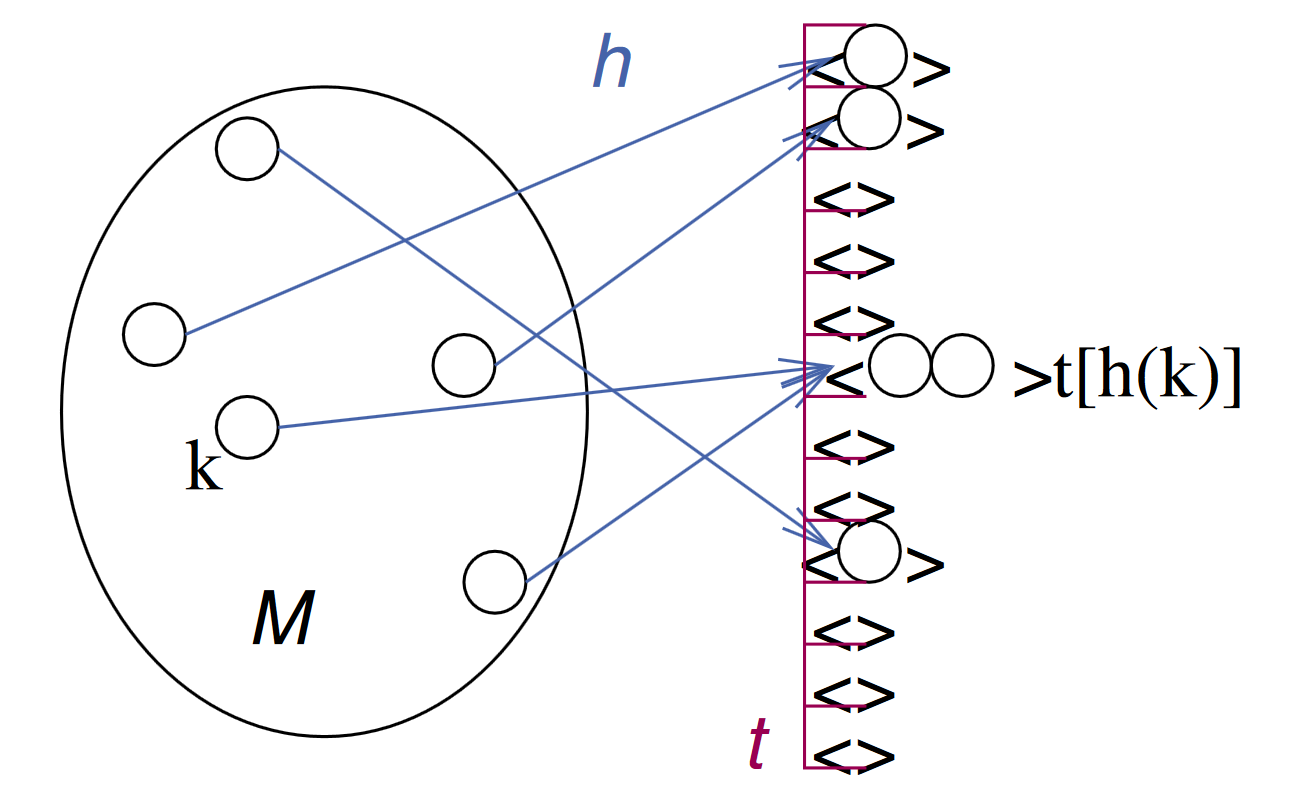
\includegraphics[width=.6\textwidth]{hashing-linked-lists}}
\end{frame}

\begin{frame}{Hashfunktionen allgemein}
	\textbf{Bearbeitungshinweise}
	\begin{itemize}
		\item Universelle Hashfunktion „herbeibeschwören“ \\
		{\small (z.B. auf Übungsblatt, in Klausur)}: \\
		„Sei h eine beliebige Hashfunktion aus der Familie universeller Hashfunktionen. Dann...“ 
		\item Ihr schreibt nen Algo. Es sollen $k$ Elemente jeweils in erwartet $O(1)$ in eine Hashtable eingefügt werden. \\
		\§{\impl} \textbf{Explizit} angeben, dass Größe der Hashtable in $\Omega(k)$ liegt! \\
		\. Sonst: Laufzeit \bfalert{kaputt}, Satz aus VL greift dann \textbf{nicht}!
	\end{itemize}
\end{frame}


\begin{frame}{Hashtables mit verketteten Listen}
	\textbf{Operation: $\|insert|(e : \Element)$} \\[0,125cm]
	\begin{itemize}
		\item Fügt das Element $e$ an den \textbf{Anfang} der Liste beim Array-Index $h(\key(e))$ ein
		\pause
		\item Erwartete Laufzeit: $O(1)$
		\item Worst-Case: $O(1)$
	\end{itemize}
\end{frame}

\begin{frame}{Hashtables mit verketteten Listen}
	\textbf{Operation: $\|remove|(k : \Z)$} \\[0,125cm]
	\begin{itemize}
		\item Entfernt das Element $e$ mit $\key(e) = k$ aus der Liste beim Array-Index $h(k)$ (und gibt $e$ zurück)
		\pause
		\item Erwartete Laufzeit: $O(1)$
		\item Worst-Case: $O(n)$
	\end{itemize}
\end{frame}

\begin{frame}{Hashtables mit verketteten Listen}
	\textbf{Operation: $\|find|(k : \Z)$} \\[0,125cm]
	\begin{itemize}
		\item Sucht das Element $e$ mit $\key(e) = k$ aus der Liste beim Array-Index $h(k)$ und gibt $e$ zurück
		\pause
		\item Erwartete Laufzeit: $O(1)$
		\item Worst-Case: $O(n)$
	\end{itemize}
\end{frame}


\begin{frame}{Hashtables mit verketteten Listen}
	\taskheading{Verkettete Listen}
	Gegeben sei eine Hashtabelle der Größe $m$ mit der Hashfunktion $h(x) := x \mod m$. Füge nacheinander folgende Elemente ein: \\ 
	36, 78, 50, 1, 92, 15, 43, 99, 64 \quad  (hierbei gilt $\key(e) := e$) \\
	Dabei sei $m$ zunächst 5 und danach 7.
\end{frame}

\begin{frame}{Hashtables mit verketteten Listen}
	\solutionheading
	$m = 5:$
	\begin{tabular}{ | c | c | c | c | c | }
		\hline
		0 & 1 & 2 & 3 & 4
		\\ \hline
		$\langle 15, 50 \rangle$ & $\langle 1,36 \rangle$ & $\langle 92 \rangle$ & $\langle 43,78 \rangle$ & $\langle 64,99 \rangle$
		\\ \hline
	\end{tabular}
	\\[0,64cm]
	$m = 7:$
	\begin{tabular}{ | c | c | c | c | c | c | c |}
		\hline
		0 & 1 & 2 & 3 & 4 & 5 & 6
		\\ \hline
		$\langle  \rangle$ & $\langle 64, 99, 43, 15, 92, 1, 50, 78, 36 \rangle$ & $\langle  \rangle$ & $\langle  \rangle$ & $\langle  \rangle$ & $\langle  \rangle$ & $\langle  \rangle$
		\\ \hline
	\end{tabular}
	\\[0,5cm]
	Achtung: Die Reihenfolge innerhalb der verketteten Liste entspricht jeweils der \textbf{umgekehrten} Einfügereihenfolge (da Elemente immer am \textbf{Anfang} der verketteten Liste hinzugefügt werden) 
\end{frame}

\section{\dots mit linearer Suche}

\begin{frame}{Hashtables mit linearer Suche}
	\begin{itemize}
		\item Verkettete Listen nicht \textit{cachefreundlich} \impl Geht es auch \textbf{ohne}?
		\pause
		\implitem Weg mit den Listen, stattdessen:
		\pause 
		\item \textbf{Einfügen}: \\ 
		Slot \textbf{besetzt}? \\ 
		\impl lege Element beim \textbf{nächstbesten} freien Slot rechts davon ab\\
		\pause
		Rechts \textbf{alles besetzt}? Zwei Möglichkeiten: \\ 
		\begin{enumerate}
			\item[1.] Array \textbf{zyklisch}: Beginne Suche von vorn 
			\item[2.] Erweitere das Array um „\textbf{Pufferbereich}“ mit Größe $m'$ \\ (auf den die Hashfunktion \textbf{nicht} abbildet)
		\end{enumerate}
		\pause
		\item \textbf{Suche}: Starte Suche wo vermutet, weiterlaufen (und testen) bis $e$ gefunden (falls $\bot$ erreicht: Abbruch)
		\pause
		\item \textbf{Entfernen}: Suche das zu entfernende Element (wie oben), danach alle Elemente, die zu weit rechts liegen, nach links schieben (\impl~Leerstellen schließen!)
	\end{itemize}
\end{frame}


\begin{frame}{Hashtables mit linearer Suche}
	\taskheading{Lineare Suche}
	Gegeben sei eine Hashtabelle der Größe $m = 8$ und Puffergröße $m' = 2$ mit der Hashfunktion $h(x) := x \mod m$. Füge nacheinander folgende Elemente ein: \\ 36, 78, 50, 1, 92, 15, 43, 99, 64 \quad (hierbei gilt $\key(e) := e$) \\
	Verwendet hierbei Hashing mit linearer Suche. \\ 
	Was passiert, wenn im Anschluss die 43 wieder entfernt wird?
\end{frame}

\begin{frame}{Hashtables mit linearer Suche}
	\solutionheading
	\begin{tabular}{ l | c | c | c | c | c | c | c | c | c | c |}
		& \multicolumn{8}{ c |}{\small m} & \multicolumn{2}{c}{\small m'}
		\\ \hline
		Index & 0 & 1 & 2 & 3 & 4 & 5 & 6 & 7 & --- & ---
		\\ \hline
		Inhalt & 64 & 1 & 50 & 43 & 36 & 92 & 78 & 15 & 99 &
		\\ \hline
	\end{tabular}
	\\[0,5cm]
	remove(43): \\
	43 entfernt, stelle fest: 99 gehört eigentlich an Slot 3! \\
	\impl verschiebe $99 \rightsquigarrow $ Slot 3. Also: \\[.3\baselineskip]
	\begin{tabular}{ l | c | c | c | c | c | c | c | c | c | c |}
		& \multicolumn{8}{ c |}{\small m} & \multicolumn{2}{c}{\small m'}
		\\ \hline
		Index & 0 & 1 & 2 & 3 & 4 & 5 & 6 & 7 & --- & ---
		\\ \hline
		Inhalt & 64 & 1 & 50 & \textbf{99} & 36 & 92 & 78 & 15 &  &
		\\ \hline
	\end{tabular}
\end{frame}

\begin{frame}{Hashtables}
	\textbf{Lineare Suche besser als Verkettete Listen?} \\[0,125cm]
	\begin{itemize}
		\pause
		\item[\Pros] Cachefreundlich 
		\pause
		\item[\Cons] Beschränkte Größe (Unbounded Array geht auch, aber mehr Sonderfälle)
		\pause
		\item[\Cons] \emph{insert} im Worst-Case in $\Theta(n)$ \\
		 Worst-Case wahrscheinlicher, weil potenziell mehr zu durchlaufen!
	\end{itemize}
\end{frame}

\begin{frame}{Hashtables}
	\ThisHasSubtasks
	\taskheading{Ein philosophischer Abend}
	
	Nach dem dritten Glas Vollmilch kommt ein Kommilitone auf die bahnbrechende Entdeckung, dass sich Hashing mit verketteten Listen hochgradig optimieren ließe, indem man die verketteten Listen stets sortiert halte. 
	\medskip
	
	Wie ändert sich das Worst-Case-Laufzeitverhalten von $insert$, $remove$ und $find$?
\end{frame}

\begin{frame}{Hashtables}
	\solutionheading
	
	\begin{itemize}
		\item $insert$: \textbf{Worst-Case} ändert sich zu $\Theta(n)$, wenn ein Element ganz am Ende eingefügt werden muss (und somit die ganze verkettete Liste durchlaufen wird)
		\item $remove$ und $find$: \textbf{Binäre Suche} wäre ne Idee, aber bringt nichts: \\
		Index-Zugriff auf Listen nicht in $O(1)$ \impl binäre Suche nicht in $O(\log n)$
	\end{itemize}
\end{frame}


\begin{frame}{Hashtables}
	\subtaskheading{Ein philosophischer Abend}
	
	Nachdem ihr einen gewissen Kommilitonen gefesselt und geknebelt auf dem Hinterhof zum Nachdenken abgelegt habt, diskutiert ihr, was passiert, wenn man die sortierten verketteten Listen durch sortierte unbeschränkte Arrays ersetzt.
	\medskip
	
	Wie ändert sich nun das Worst-Case-Laufzeitverhalten von $insert$, $remove$ und $find$?
\end{frame}

\begin{frame}{Hashtables}
	\solutionheading
	\begin{itemize}
		\item $insert$: Im Worst-Case immer noch $\Theta(n)$. Zwar kann die Einfügestelle mit binärer Suche in $\Theta( \log n)$ gefunden werden, doch alle Elemente rechts davon müssen um eins verschoben werden
		\pause
		\item $remove$: Auch weiterhin $\Theta(n)$. Binäre Suche hilft zwar beim Finden, aber alle Nachfolger müssen um eins nach links aufrücken
		\pause
		\item $find$: Binäre Suche bringt „endlich“ etwas \impl Laufzeit $\Theta( \log n)$
	\end{itemize}
\end{frame}


\begin{frame}{Hashtables}
	\subtaskheading{Ein philosophischer Abend}
	
	Da außer euch zur späten Stunde keine anderen Kunden mehr vorhanden sind, gesellt sich der Milchbarkeeper zu euch und fragt, ob man da nicht noch was mit amortisierter Analyse machen kann.
	\medskip
	
	Welches amortisierte Laufzeitverhalten lässt sich für $insert$, $remove$ und $find$ diagnostizieren (wenn man weiterhin sortierte unbeschränkte Arrays verwendet)?
\end{frame}

\begin{frame}{Hashtables}
	\solutionheading
	\begin{itemize}
		\item $insert$: Betrachte eine Folge von $n$ Einfügeoperationen, deren Elemente streng monoton kleiner werden (Worst-Case). Die $k$-te Einfügeoperationen muss $(k-1)$ Elemente verschieben \\
		\impl n Operationen haben die Laufzeit $\Theta(n^2)$, da lässt sich nichts amortisieren
		\pause
		\item $remove$: Zunächst ähnlich wie bei $insert$. \\
		Aber: Zu jedem \emph{remove} in $O(n)$ gehört auch ein \emph{insert} in $O(n)$. Also: Wälze den Aufwand von $remove$ auf $insert$ ab \\ \impl $remove$ läuft amortisiert in $O(1)$. {\small (Anmerkung: Einen praktischen Nutzen hat diese Betrachtungsweise leider nicht wirklich.)}
		\pause
		\item 	$find$: Hat immer die Laufzeit $\Theta(\log n)$, daran ändert auch Amortisierung nichts.
	\end{itemize}
\end{frame}



\begin{frame}{Komplexe Datenstrukturen}
	\taskheading{SparseArray}
	Nehmt an, dass \textbf{allocate} euch beliebig viel \emph{uninitialisierten} Speicher in konstanter Zeit liefert. Entwerft anhand dessen ein \emph{SparseArray} mit folgenden Eigenschaften: 
	\begin{itemize}
		\item Ein \emph{SparseArray} mit $n$ Slots braucht $O(n)$ Speicher
		\item Die Erzeugung eines leeren Arrays mit $n$ Slots braucht $O(1)$ Zeit
		\item Eine Operation $reset$, die das \emph{SparseArray} in $O(1)$ Zeit in leeren Zustand versetzt
		\item Die Operationen $get(i)$ und $set(i, x)$, die Zugriff auf den Inhalt am entspr. Index in $O(1)$ gewährleisten. Falls dieser leer ist, soll $\bot$ zurückgeliefert werden.
	\end{itemize}
\end{frame}

\begin{frame}{Komplexe Datenstrukturen}
	\solutionheading
	
	Konstruiere ein \emph{SparseArray} der Größe $n$ mihtilfe von drei Arrays: \\ 
	$D$ (für die \textbf{Daten}), $Z$ (für \textbf{Zähler}) und $B$ (für \textbf{Beweise}). \\ 
	Zudem initialisiere Counter $c := 0$. \\ 
	\impl \textbf{Speicheraufwand} in $O(n)$, \textbf{Erzeugung} läuft in $O(1)$ weil Speicherallokation in $O(1)$. \\
	Operationen: \\
	\pause
	\begin{columns}[c]
		\column[T]{.3\textwidth}
		\begin{algorithm}[H]
			\Procedure{set$(i, x)$}{
				$D[i] := x$ \;
				$Z[i] := c$ \;
				$B[c] := i$ \;
				$c\pp$ 
			}
		\end{algorithm}
		\column[T]{.64\textwidth}
		\forcenewline
			(Durch $Z$ und $B$ entsteht somit ein rückversichernder Zirkelbezug, und $c$ garantiert uns, bis zu welchem Index die Daten in $B$ valide sind, d.h., $B[0...c-1]$ enthält alle gültigen Indizes).
	\end{columns}
	
	
\end{frame}

\begin{frame}{Komplexe Datenstrukturen}
	\solutionheading
	
	\begin{algorithm}[H]
		\Function{get$(i)$}{
			\eIf{$Z[i] < c \KwAnd B[Z[i]] = i$}{
				\Return{$D[i]$}
			}{
				\LComment{garbage inside $D[i]$, so:} \;
				\Return{$\bot$} 
			}
		}
		\;
		\pause
		\;
		\Procedure{reset}{
			$c := 0$ \;
			\LComment{Das markiert recht gemütlich den Inhalt aller Arrays als Unsinn}
		}
	\end{algorithm}
\end{frame}

\xkcdframevert{795}{Danke für die Aufmerksamkeit! \smiley}{2}

\end{document}